% !TEX TS-program = pdflatex
\documentclass[11pt]{article}

% -------------------- Packages --------------------
\usepackage[a4paper,margin=1in]{geometry}
\usepackage{amsmath,amssymb}
\usepackage[T1]{fontenc}
\usepackage{lmodern}
\usepackage{xcolor}
\usepackage{tcolorbox}
\tcbuselibrary{skins,breakable}
\usepackage{enumitem}
\usepackage{hyperref}
\usepackage{tikz}
\usetikzlibrary{calc,angles,quotes}

\pagestyle{empty}

% -------------------- Dark Theme Colors --------------------
\definecolor{bg}{HTML}{000000}
\definecolor{pairbg}{HTML}{121212}
\definecolor{solbg}{HTML}{0A0A0A}
\definecolor{border}{HTML}{2A2A2A}
\definecolor{text}{HTML}{FFFFFF}
\definecolor{muted}{HTML}{C9CDD3}
\definecolor{gold}{HTML}{FFD700}
\definecolor{green}{HTML}{4ADE80}
\definecolor{cyan}{HTML}{38BDF8}

\pagecolor{bg}
\color{text}

\hypersetup{
  colorlinks=true,
  linkcolor=cyan,
  urlcolor=cyan
}

\setlength{\parindent}{0pt}
\setlength{\parskip}{10pt}

\setlist[itemize]{left=1.4em,itemsep=6pt,topsep=6pt}
\setlist[enumerate]{left=1.6em,itemsep=4pt,topsep=4pt}

% -------------------- tcolorbox Base --------------------
\tcbset{
  enhanced,
  breakable,
  arc=12pt,
  boxrule=0.8pt,
  left=16pt,right=16pt,top=12pt,bottom=12pt
}

\newtcolorbox{QAPair}[1]{%
  colback=pairbg,
  colbacklower=solbg,
  colframe=border,
  coltext=text,
  title=\textcolor{gold}{\bfseries #1},
  fonttitle=\bfseries,
  coltitle=text,
  segmentation style={draw=border, dashed, line width=0.6pt},
}

\newtcolorbox{QuickBox}{%
  colback=pairbg,
  colframe=cyan,
  coltext=text,
  fontupper=\color{text},
  borderline north={4pt}{0pt}{cyan},
  arc=14pt,
  boxrule=0.8pt
}

% Helper for step headings
\newcommand{\Step}[1]{\textcolor{muted}{\textbf{Step #1:}}}

% ============================================================
\begin{document}

\begin{center}
{\LARGE\bfseries \textcolor{gold}{Exercise 9.6 --- Solutions}}\\[-2pt]
\end{center}

\begin{QuickBox}
{\color{cyan}\bfseries Quick formulas (useful)}\par\medskip
\begin{itemize}
\item \textbf{Equilateral triangle:} $P=3s$.
\item \textbf{Parallelogram area:} $A=\text{base}\times\text{height}$.
\item \textbf{Regular $n$-gon:} $P=ns$, \quad $A=\dfrac12(\text{apothem})\cdot P$.
\item \textbf{Regular hexagon area:} $A=\dfrac{3\sqrt3}{2}s^2$.
\item \textbf{Square:} if $P=4s$ then $s=\dfrac{P}{4}$ and $A=s^2$.
\item \textbf{Unit conversion (used in Q5):} $1\text{ ft}=0.3048\text{ m}$, hence $1\text{ ft}^2=(0.3048)^2\approx 0.092903\text{ m}^2$.
\end{itemize}
\end{QuickBox}

% ============================================================
% Q1
\begin{QAPair}{Question 1}
\textcolor{gold}{\bfseries Question:} A lawn is in the shape of an equilateral triangle. Find the perimeter of lawn if length of one side is $5\text{ m}$. Also find the cost of boundary wall of lawn @ Rs.\ 220 per metre.

\begin{center}
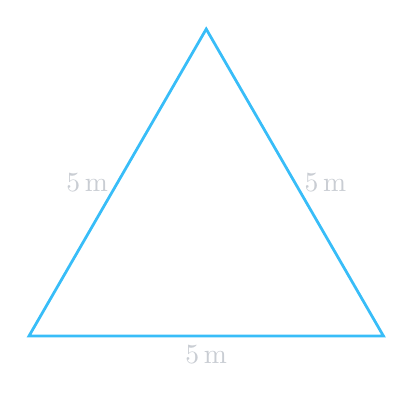
\begin{tikzpicture}[scale=0.9]
\coordinate (A) at (0,0);
\coordinate (B) at (5,0);
\coordinate (C) at (2.5,4.33);
\draw[cyan, line width=1pt] (A)--(B)--(C)--cycle;
\node[below,text=muted] at ($(A)!0.5!(B)$) {$5\,\text{m}$};
\node[left,text=muted]  at ($(A)!0.5!(C)$) {$5\,\text{m}$};
\node[right,text=muted] at ($(B)!0.5!(C)$) {$5\,\text{m}$};
\end{tikzpicture}
\end{center}

\tcblower
\textcolor{green}{\bfseries Answer:}
\[
\begin{aligned}
\Step{1}\;& \text{Equilateral triangle}\Rightarrow P=3s=3(5)=15\ \text{m}.\\
\Step{2}\;& \text{Cost of boundary wall }=P\times 220=15\times 220=3300.\\[2pt]
&\boxed{P=15\ \text{m}},\qquad \boxed{\text{Cost}= \text{Rs.\ }3300}.
\end{aligned}
\]
\end{QAPair}

% ============================================================
% Q2
\begin{QAPair}{Question 2}
\textcolor{gold}{\bfseries Question:} Cricket ground in a village is in the shape of a parallelogram. One side of ground is $65\text{ m}$ long and distance between parallel sides having length $65\text{ m}$ is $42\text{ m}$. Find the cost of planting grass @ Rs.\ 10 per square metre.

\begin{center}
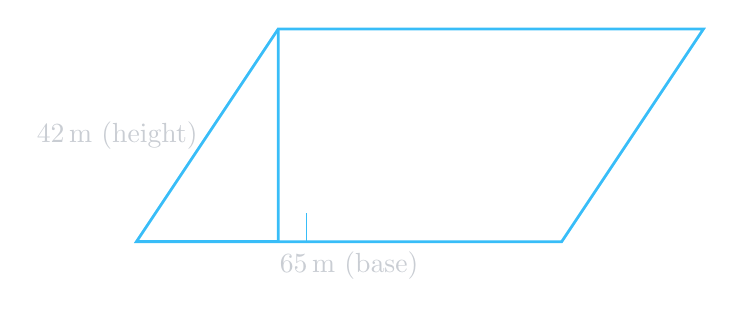
\begin{tikzpicture}[scale=0.9]
\coordinate (A) at (0,0);
\coordinate (B) at (6,0);
\coordinate (C) at (8,3);
\coordinate (D) at (2,3);
\draw[cyan, line width=1pt] (A)--(B)--(C)--(D)--cycle;
\draw[cyan, dashed] (D)--(A);
\draw[cyan] (D) -- ($(D)!1!(A)$);
\draw[cyan, line width=1pt] (D) -- (2,0);
\draw[cyan, line width=1pt] (2,0) -- (A);
\node[below,text=muted] at ($(A)!0.5!(B)$) {$65\,\text{m}$ (base)};
\node[left,text=muted]  at ($(A)!0.5!(D)$) {$42\,\text{m}$ (height)};
% little right angle
\draw[cyan] (2,0) -- (2.4,0) -- (2.4,0.4);
\end{tikzpicture}
\end{center}

\tcblower
\textcolor{green}{\bfseries Answer:}
\[
\begin{aligned}
\Step{1}\;& A=\text{base}\times\text{height}=65\times 42=2730\ \text{m}^2.\\
\Step{2}\;& \text{Cost}=A\times 10=2730\times 10=27300.\\[2pt]
&\boxed{A=2730\ \text{m}^2},\qquad \boxed{\text{Cost}= \text{Rs.\ }27300}.
\end{aligned}
\]
\end{QAPair}

% ============================================================
% Q3
\begin{QAPair}{Question 3}
\textcolor{gold}{\bfseries Question:} Base of a minaret of a Masjid is built in the shape of regular pentagon as shown in the figure. Find the perimeter and area of base of minaret.

\begin{center}
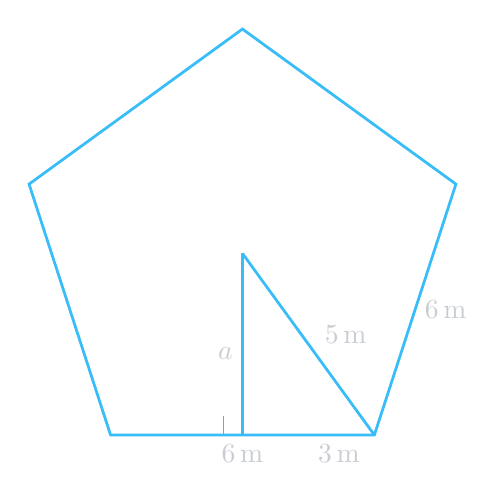
\begin{tikzpicture}[scale=0.95]
% Regular pentagon (approx)
\coordinate (O) at (0,0);
\foreach \k/\name in {90/A,18/B,-54/C,-126/D,162/E}{
  \coordinate (\name) at ({3*cos(\k)},{3*sin(\k)});
}
\draw[cyan, line width=1pt] (A)--(B)--(C)--(D)--(E)--cycle;

% Base side and midpoint
\coordinate (M) at ($(C)!0.5!(D)$);
% Draw apothem
\draw[cyan, line width=1pt] (O)--(M);
% Draw radius to a vertex
\draw[cyan, line width=1pt] (O)--(C);

% Right angle mark at M
\draw[cyan] ($(M)+(0.0,0.0)$) -- ++(-0.25,0) -- ++(0,0.25);

% Labels (given in picture style)
\node[below,text=muted] at ($(C)!0.5!(D)$) {$6\,\text{m}$};
\node[right,text=muted] at ($(B)!0.5!(C)$) {$6\,\text{m}$};

% Small right triangle idea: half side = 3m, radius = 5m, apothem = a
\coordinate (H) at ($(M)!0.0!(C)$); % same as M
\coordinate (P) at ($(C)!0.5!(D)$); % M already
% Show half-side on base (M to C is 3m conceptually)
\draw[cyan] (M)--(C);
\node[below right,text=muted] at ($(M)!0.5!(C)$) {$3\,\text{m}$};

% Radius label (O to C)
\node[above right,text=muted] at ($(O)!0.55!(C)$) {$5\,\text{m}$};

% Apothem label
\node[left,text=muted] at ($(O)!0.55!(M)$) {$a$};
\end{tikzpicture}
\end{center}

\tcblower
\textcolor{green}{\bfseries Answer:}
\[
\begin{aligned}
\Step{1}\;& \text{From the figure: side } s=6\text{ m} \Rightarrow P=5s=5(6)=30\text{ m}.\\
\Step{2}\;& \text{Find apothem }a:\ \text{right triangle with } \frac{s}{2}=3,\ \text{hypotenuse }=5.\\
& a=\sqrt{5^2-3^2}=\sqrt{25-9}=\sqrt{16}=4\ \text{m}.\\
\Step{3}\;& \text{Area of regular polygon }A=\frac12 aP=\frac12(4)(30)=60\ \text{m}^2.\\[2pt]
&\boxed{P=30\ \text{m}},\qquad \boxed{A=60\ \text{m}^2}.
\end{aligned}
\]
\end{QAPair}

% ============================================================
% Q4
\begin{QAPair}{Question 4}
\textcolor{gold}{\bfseries Question:} A plot in the shopping area is in the shape of regular hexagon. One side of the plot is $10\text{ m}$ long. Find:
\begin{enumerate}[label=(\roman*)]
\item the cost of fencing the plot @ Rs.\ 160 per metre.
\item area of the plot.
\item the cost of filling the plot @ Rs.\ 500 per m$^2$.
\end{enumerate}

\begin{center}
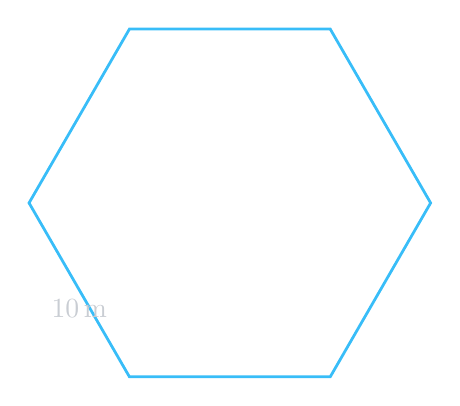
\begin{tikzpicture}[scale=0.85]
\coordinate (O) at (0,0);
\foreach \k [count=\i] in {0,60,120,180,240,300}{
  \coordinate (P\i) at ({3*cos(\k)},{3*sin(\k)});
}
\draw[cyan, line width=1pt] (P1)--(P2)--(P3)--(P4)--(P5)--(P6)--cycle;
\node[below,text=muted] at ($(P4)!0.5!(P5)$) {$10\,\text{m}$};
\end{tikzpicture}
\end{center}

\tcblower
\textcolor{green}{\bfseries Answer:}
\[
\begin{aligned}
\Step{1}\;& s=10\text{ m}\Rightarrow P=6s=6(10)=60\text{ m}.\\
\Step{2}\;& \text{Fencing cost}=P\times 160=60\times 160=9600.\\[4pt]
\Step{3}\;& \text{Area of regular hexagon: }A=\frac{3\sqrt3}{2}s^2
=\frac{3\sqrt3}{2}(10^2)=150\sqrt3\ \text{m}^2\\
&\hspace{2.7em}\approx 150(1.732)=259.8\ \text{m}^2.\\[4pt]
\Step{4}\;& \text{Filling cost}=A\times 500=(150\sqrt3)\times 500=75000\sqrt3\\
&\hspace{2.7em}\approx 259.8\times 500=129900.\\[2pt]
&\boxed{\text{(i) Rs.\ }9600},\quad
\boxed{\text{(ii) }A=150\sqrt3\approx 259.8\ \text{m}^2},\quad
\boxed{\text{(iii) Rs.\ }75000\sqrt3\approx 129900}.
\end{aligned}
\]
\end{QAPair}

% ============================================================
% Q5
\begin{QAPair}{Question 5}
\textcolor{gold}{\bfseries Question:} A room is in the shape of square having perimeter of $48$ feet. Find:
\begin{enumerate}[label=(\roman*)]
\item the cost of carpeting the floor @ Rs.\ 350 per m$^2$.
\item the inner area of each wall if room is $10$ feet high.
\item the cost of painting inner sides of the room @ Rs.\ 100 per m$^2$.
\end{enumerate}

\begin{center}
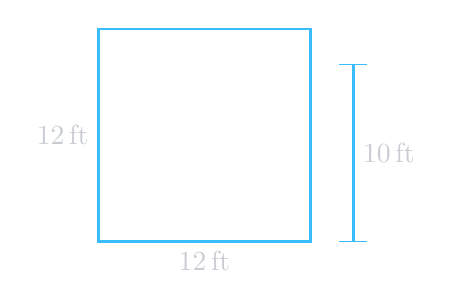
\begin{tikzpicture}[scale=0.9]
\draw[cyan, line width=1pt] (0,0) rectangle (3,3);
\node[below,text=muted] at (1.5,0) {$12\,\text{ft}$};
\node[left,text=muted]  at (0,1.5) {$12\,\text{ft}$};
% wall height indicator
\draw[cyan, line width=1pt] (3.6,0) -- (3.6,2.5);
\draw[cyan] (3.4,0) -- (3.8,0);
\draw[cyan] (3.4,2.5) -- (3.8,2.5);
\node[right,text=muted] at (3.6,1.25) {$10\,\text{ft}$};
\end{tikzpicture}
\end{center}

\tcblower
\textcolor{green}{\bfseries Answer:}
\[
\begin{aligned}
\Step{1}\;& \text{Square perimeter }P=4s=48\Rightarrow s=\frac{48}{4}=12\ \text{ft}.\\[2pt]
\Step{2}\;& \text{Floor area}=s^2=12^2=144\ \text{ft}^2.\\
&\text{Convert: }1\ \text{ft}^2\approx 0.092903\ \text{m}^2\\
&\Rightarrow A_{\text{floor}}\approx 144(0.092903)=13.378\ \text{m}^2.\\
&\text{Carpet cost}\approx 13.378\times 350=4682.3\ \Rightarrow\ \boxed{\text{Rs.\ }4682\ (\text{approx})}.\\[6pt]
\Step{3}\;& \text{Each wall area}=(\text{width})(\text{height})=(12)(10)=120\ \text{ft}^2\\
&\Rightarrow A_{\text{one wall}}\approx 120(0.092903)=11.148\ \text{m}^2.\\
&\boxed{A_{\text{each wall}}\approx 11.15\ \text{m}^2}.\\[6pt]
\Step{4}\;& \text{Total inner wall area (4 walls)}=4\times 120=480\ \text{ft}^2\\
&\Rightarrow A_{\text{walls}}\approx 480(0.092903)=44.593\ \text{m}^2.\\
&\text{Painting cost}\approx 44.593\times 100=4459.3\Rightarrow \boxed{\text{Rs.\ }4459\ (\text{approx})}.
\end{aligned}
\]
\end{QAPair}

% ============================================================
% Q6
\begin{QAPair}{Question 6}
\textcolor{gold}{\bfseries Question:} A tile is in the shape of regular hexagon. Each side of the tile is one foot long. Find the perimeter of four tiles joined together as shown in the figure.

\begin{center}
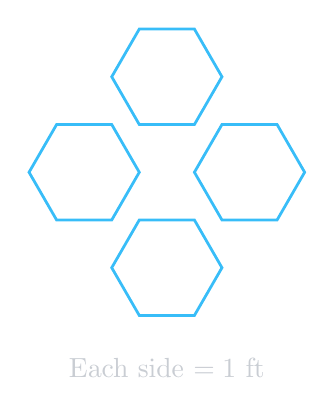
\begin{tikzpicture}[scale=0.7]
% helper: draw a hexagon centered at (x,y) with side 1 (circumradius 1)
\newcommand{\drawhex}[2]{%
  \begin{scope}[shift={(#1,#2)}]
    \foreach \k [count=\i] in {0,60,120,180,240,300}{
      \coordinate (H\i) at ({cos(\k)},{sin(\k)});
    }
    \draw[cyan, line width=1pt] (H1)--(H2)--(H3)--(H4)--(H5)--(H6)--cycle;
  \end{scope}
}
% Arrange 4 hexagons (top, bottom, left, right) around a central gap
\drawhex{0}{1.732}   % top
\drawhex{0}{-1.732}  % bottom
\drawhex{-1.5}{0}    % left
\drawhex{1.5}{0}     % right

\node[below,text=muted] at (0,-3.2) {Each side $=1$ ft};
\end{tikzpicture}
\end{center}

\tcblower
\textcolor{green}{\bfseries Answer:}
\[
\begin{aligned}
\Step{1}\;& \text{One hexagon has }6\text{ sides, each }1\text{ ft}\Rightarrow P_1=6\text{ ft}.\\
\Step{2}\;& \text{For 4 tiles, total sides }=4\times 6=24\ \text{(ft-edges)}.\\
\Step{3}\;& \text{In the given arrangement, there are }4\text{ shared sides (internal).}\\
&\text{Each shared side removes }2\text{ edges from the outside perimeter.}\\
\Step{4}\;& P_{\text{joined}}=24-2(4)=24-8=16\ \text{ft}.\\[2pt]
&\boxed{P=16\ \text{ft}}.
\end{aligned}
\]
\end{QAPair}

\end{document}
